\documentclass[dvipdfmx]{jsarticle}
\usepackage[T1]{fontenc}
\usepackage[dvipdfmx]{hyperref}
\usepackage{lmodern}
\usepackage{latexsym}
\usepackage{amsfonts}
\usepackage{amssymb}
\usepackage{mathtools}
\usepackage{amsthm}
\usepackage{multirow}
\usepackage[dvipdfmx]{graphicx}
\usepackage{wrapfig}
\usepackage{here}
\usepackage{float}
\usepackage{ascmac}
\usepackage{url}

\title{人物相関図の可視化-課題研究3-}
\author{文理学部情報科学科\\5419045 高林 秀}
\date{\today}

\begin{document}

\maketitle

\begin{abstract}
本稿は、今年度コンピューティング2のネットワークの可視化に関する課題として、小説レ・ミゼラブルの人物相関図をグラフで可視化する実験を行うものである。なお、本課題ではprocessing for javaを使用した。
\end{abstract}

\section{目的}
本稿は、今年度コンピューティング2の課題研究として「ネットワークの可視化」に関する問題に解答するものである。また同時に、問題に関する計算理論についても復習するものとする。
\section{計算理論}
今回の実験で使用したForce-directedアルゴリズムについて、関連する用語もセットで説明する。
\subsection{グラフ描画について}
数学的なグラフ理論におけるグラフは、ノードの集合とノード間を結ぶ辺、すなわちリンクより成立している。グラフはノード間のつながりという関係のみを持つが、グラフの構造までは2,3次元に描画してみないと視覚化することができない。画面にノードとリンクを直接的に描画した図をノードリンク図と呼ぶ。\par
ノードリンク図を描画するにあたって、ノードを画面上のどの位置に描画させるか決定しなければならない。すなわち、グラフの描画とはノードの画面上での位置を決定する操作を指す。\par
一般に、グラフのどの特徴を描画するかによってグラフ描画の手法は異なってくる。グラフ描画によって可視化されるグラフ構造は様々なネットワークや、データ構造の理解に役立てることが可能である。
\begin{figure}[H]
  \centering
  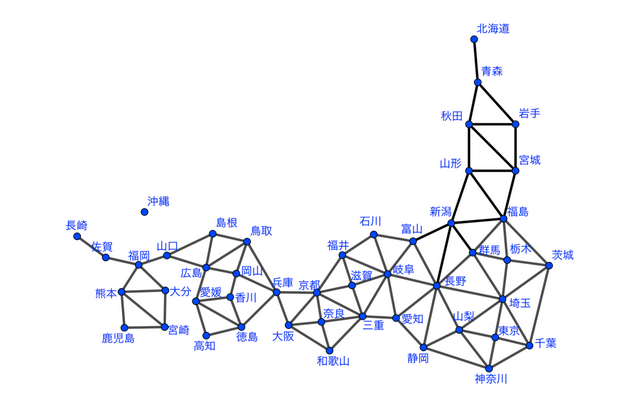
\includegraphics[scale=0.4]{images/graph_img.png}
  \caption{グラフ描画の例}
  出典:\url{https://qiita.com/drken/items/4a7869c5e304883f539b}
\end{figure}
グラフをプログラム上で考えるとき各ノードについて、ノードの個数分の座標と速度を配列に保持しておく必要がある。これは、複数の物体の運動と同じである。リンクに関しては、どのノードとどのノードが接続されているか片方のノードの添字sorceともう片方のノードの添字targetをそれぞれ整数型の配列で表現することになる。\par
ノード間のリンクをバネと見なして、その運動をシミュレーションし描画する。このように、リンクをバネと見なしてグラフ描画を行うことをバネモデルと呼ぶ。バネモデルの有名なグラフ描画として、Eadasの方法が挙げられる。Eadasの方法に関して本稿では、詳細な説明は扱わないが、下記のリンクを参照いただきたい。
\begin{itemize}
  \item Eadasの方法:\url{http://www2.kobe-u.ac.jp/~ky/labo/research/graph-drawing.htm}
\end{itemize}
本稿では、後述するVerlet法により実現できるバネモデルの描画を行う。\par
\subsection{Force-directedアルゴリズム}
グラフ描画の手法の1つとして、Force-directedアルゴリズムが存在する。このアルゴリズムは、ノード間に作用する力をシミュレーションすることによりノードの座標を決定する。ノード間のリンクをバネと見なして、その運動をシミュレーションし描画する。\par
バネモデルをシミュレーションするにはまず、ノードの初期座標を適当に与える必要がある。このときrandom()関数を利用し初期位置を任意に決定することができる。次に、全リンクに対しフックの法則\footnote{1687年にイギリスのR・フックにより発見された物理法則。バネのような弾性をもつ物体に力を加えて変形させると、変形の小さい間は力と変形が比例する、つまり弾性状態では応力とひずみが比例関係にあるという法則。$\sigma を応力、Eをヤング率、\epsilon をひずみとすると、\sigma = E\epsilon$と示せる・}に従う力の計算を行う。しかしそれだけでは座標は収束しない。したがって、空気抵抗を計算しノードの座標が静止状態になるまで繰り返し計算を行う。なお、ノードが描画範囲から大きく外れることも考えられるので、速度更新のときは全ノードの重心が描画領域の中央に来るようノード座標の平行移動を行う。\par
以下は、完全グラフ$K_{3}$のバネモデルを可視化したp5.jsコードである。
\begin{verbatim}
  const n = 3;
  const x = new Array(n);
  const y = new Array(n);
  const vx = new Array(n);
  const vy = new Array(n);
  const r = 25;

  const m = 3;
  const source = [0, 0, 1];
  const target = [1, 2, 2];

  function setup() {
    createCanvas(600, 600);
    for (let i = 0; i < n; ++i) {
      x[i] = random(width);
      y[i] = random(height);
    }
    vx.fill(0);
    vy.fill(0);
  }

  function draw() {
    drawObjects();
    updatePosition();
    updateVelocity();
  }

  function drawObjects() {
    background(255);
    for (let i = 0; i < m; ++i) {
      const s = source[i];
      const t = target[i];
      line(x[s], y[s], x[t], y[t]);
    }
    for (let i = 0; i < n; ++i) {
      fill(255);
      ellipse(x[i], y[i], 2 * r, 2 * r);
      fill(0);
      textSize(32);
      textAlign(CENTER, CENTER);
      text(i, x[i], y[i]);
    }
  }

  function updatePosition() {
    for (let i = 0; i < n; ++i) {
      x[i] += vx[i];
      y[i] += vy[i];
    }
  }

  function updateVelocity() {
    applySpringForce(0.001, 200);
    applyResistanceForce(0.01);
    applyCentering();
  }

  function applySpringForce(k, L) {
    for (let i = 0; i < m; ++i) {
      const s = source[i];
      const t = target[i];
      const d = dist(x[s], y[s], x[t], y[t]);
      const theta = atan2(y[s] - y[t], x[s] - x[t]);
      const w = k * (L - d);
      vx[s] += w * cos(theta);
      vy[s] += w * sin(theta);
      vx[t] -= w * cos(theta);
      vy[t] -= w * sin(theta);
    }
  }

  function applyResistanceForce(k) {
    for (let i = 0; i < n; ++i) {
      vx[i] += -k * vx[i];
      vy[i] += -k * vy[i];
    }
  }

  function applyCentering() {
    let cx = 0;
    let cy = 0;
    for (let i = 0; i < n; ++i) {
      cx += x[i];
      cy += y[i];
    }
    cx /= n;
    cy /= n;
    for (let i = 0; i < n; ++i) {
      x[i] += -cx + width / 2;
      y[i] += -cy + height / 2;
    }
  }
\end{verbatim}
この実行結果は下図。
\begin{figure}[H]
  \centering
  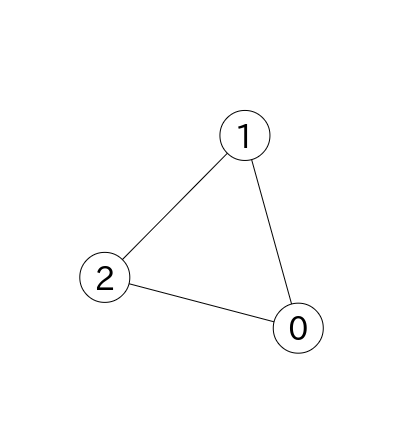
\includegraphics[scale=0.4]{images/K3result.png}
  \caption{完全グラフ$K_{3}$のバネモデル}
  出典:\url{https://qiita.com/drken/items/4a7869c5e304883f539b}
\end{figure}
下記のp5.jsコードはForce-directedアルゴリズムによって可視化したノード数10個のグラフを描画したものである。各ノードのペアは$\frac{1}{2}$の確率でリンクを持つようにランダムにグラフを生成している。
\begin{verbatim}
  let n;
  let x;
  let y;
  let vx;
  let vy;

  let m;
  let source;
  let target;

  const r = 25;

  function setup() {
    createCanvas(600, 600);
    initializeGraph(10);
    for (let i = 0; i < n; ++i) {
      x[i] = random(width);
      y[i] = random(height);
    }
    vx.fill(0);
    vy.fill(0);
  }

  function draw() {
    drawObjects();
    updatePosition();
    updateVelocity();
  }

  function initializeGraph(k) {
    n = k;
    x =  new Array(n);
    y =  new Array(n);
    vx = new Array(n);
    vy = new Array(n);
    m = 0;
    source = new Array();
    target = new Array();
    for (let i = 0; i < n; ++i) {
      for (let j = i + 1; j < n; ++j) {
        if (random(1) < 0.5) {
          source.push(i);
          target.push(j);
          m += 1;
        }
      }
    }
  }

  function drawObjects() {
    background(255);
    for (let i = 0; i < m; ++i) {
      const s = source[i];
      const t = target[i];
      line(x[s], y[s], x[t], y[t]);
    }
    for (let i = 0; i < n; ++i) {
      fill(255);
      ellipse(x[i], y[i], 2 * r, 2 * r);
      fill(0);
      textSize(32);
      textAlign(CENTER, CENTER);
      text(i, x[i], y[i]);
    }
  }

  function updatePosition() {
    for (let i = 0; i < n; ++i) {
      x[i] += vx[i];
      y[i] += vy[i];
    }
  }

  function updateVelocity() {
    applySpringForce(0.001, 10);
    applyRepulsiveForce(10);
    applyResistanceForce(0.01);
    applyCentering();
  }

  function applySpringForce(k, L) {
    for (let i = 0; i < m; ++i) {
      const s = source[i];
      const t = target[i];
      const d = dist(x[s], y[s], x[t], y[t]);
      const theta = atan2(y[s] - y[t], x[s] - x[t]);
      const w = k * (L - d);
      vx[s] += w * cos(theta);
      vy[s] += w * sin(theta);
      vx[t] -= w * cos(theta);
      vy[t] -= w * sin(theta);
    }
  }

  function applyRepulsiveForce(q) {
    for (let i = 0; i < n; ++i) {
      for (let j = 0; j < n; ++j) {
        if (i === j) {
          continue;
        }
        const d = distance(i, j);
        const w = -q / (d * d);
        vx[i] += (x[j] - x[i]) * w;
        vy[i] += (y[j] - y[i]) * w;
      }
    }
  }

  function applyResistanceForce(k) {
    for (let i = 0; i < n; ++i) {
      vx[i] += -k * vx[i];
      vy[i] += -k * vy[i];
    }
  }

  function applyCentering() {
    let cx = 0;
    let cy = 0;
    for (let i = 0; i < n; ++i) {
      cx += x[i];
      cy += y[i];
    }
    cx /= n;
    cy /= n;
    for (let i = 0; i < n; ++i) {
      x[i] += -cx + width / 2;
      y[i] += -cy + height / 2;
    }
  }

  function distance(i, j) {
    const minDistance = 10;
    const d = dist(x[i], y[i], x[j], y[j]);
    if (d < minDistance) {
      return minDistance;
    }
    return d;
  }
\end{verbatim}
\subsection{Verlet法}
\subsubsection{ニュートンの運動方程式とVerlet法}
\paragraph{ニュートンの運動方程式}
物体にかかる力を$F$、質量を$m$、加速度を$\alpha$としたとき、以下の関係を運動方程式という。
\begin{gather*}
  F = m\alpha
\end{gather*}
このとき、物体の速度を$v$としたとき$\alpha$は$v$の微分、物体の位置を$r$としたとき$v$は$r$の微分になる。したがって、運動方程式は$r$の2階微分により以下のように示すことができる。
\begin{gather*}
  \frac{d^{2}}{dt^{2}}r = \frac{F(t)}{m} = \alpha
\end{gather*}
上記式は、$\alpha$と$r$の関係性を示した微分方程式で、これを解くと物体の運動を計算することができる。また、ある時点$t$における加速度$\alpha(t)$が示されている場合、Runge-Kutta法を使用することでより高精度な解を得ることができる。ただし、ふくすうの 物体が複雑に相互作用しているような場合、解を得ることが難しくなる。\par
\paragraph{速度Verlet法}
$r(t)$の$t_{0}$まわりにおけるテイラー展開は下記のようになる。
\begin{gather*}
  r(t)\simeq r(t_{0}) + (t-t_{0})v(t_{0}) + \frac{(t-t_{0})^{2}}{2}\alpha(t_{0})
\end{gather*}
$t_{0}$から微小時間$\Delta$分だけ変化した時点の位置$r(t+\Delta)$は$t = t_{0} + \Delta$のときに得ることができる。実際に代入すると以下のようになる。
\begin{gather*}
  r(t_{0} + \Delta)\simeq r(t_{0}) + \Delta v(t_{0}) + \frac{\Delta^{2}}{2}\alpha(t_{0})
\end{gather*}
上記は、$r(t)$の更新式となる。これを整理すると、速度$v(t)$に関する更新式を得ることができる。
\begin{gather*}
  v(t_{0} L \Delta)\simeq v(t_{0}) + \frac{\Delta}{2}(\alpha (t_{0}+\Delta) + \alpha(t_{0}))
\end{gather*}
したがって、ある時点$t$における加速度$\alpha(t)$が今の位置$r(t)$によって得ることができたら、速度$v(t + \Delta)$と位置$r(t + \Delta)$を更新することができる。これを速度Verlet法という。\par
速度Verlet法は、加速度を計算して速度を更新し、その速度を利用して物体の座標を更新していく手法である。粒子の衝突を考慮する場合やm粒子にかかる力が時点ごとに変化する場合に適しており、実際の分子動力学シミュレーションで利用されている計算法である。
\subsubsection{簡易版速度Verlet法}
速度Verlet法は一般に2次のテイラー展開が利用される。しかし実際の物理現象を正確に再現するにはより高精度な精度の計算が必要になる。ただし、本稿で行うネットワークの可視化は粒子間の物理的な相互作用を隠喩にするが、現象のシミュレーションではないので精度は必要ない。したがってより簡易的なVerlet法の更新式を利用することができる。\par
1次のテイラー展開を使用して、$\Delta = 1$とすれば更新式は下記のようになる。
\begin{gather*}
  r(t + 1) = r(t) + v(t)\\
  v(t + 1) = v(t) + \alpha(t)
\end{gather*}
2次元空間上の現在の座標$r = (x, y)$と速度$v = (v_{x}, v_{y})$が得られており加速度$\alpha =(\alpha_{x}, \alpha_{y})$を計算することで、物体の座標を更新する。コード内では以下のように記載することで、更新できる。
\begin{verbatim}
  x += vx;
  y += vy;
  vx += ax;
  vy += ay;
\end{verbatim}
\section{実験方法}
\subsection{計算機環境}
本課題を解いた際の計算機環境を下記に示す。
\begin{itemize}
  \item ホストOS:Window10 Home Ver.20H2
  \item 仮想OS:Ubuntu 20.04.2 LTS
  \item CPU:Intel(R)Core(TM)i7-9700K @ 3.6GHz
  \item GPU:Nvidia Geforce RTX2070 OC @ 8GB
  \item ホストRAM:16GB
  \item 仮想RAM:4GB
\end{itemize}
\subsection{課題}
小説レ・ミセラブルにおいて、同じ章に出演する人物をグラフで表したデータが以下の5つのファイルに格納されている。
\begin{itemize}
  \item name.txt
  \item source.txt
  \item target.txt
  \item group.txt
  \item weight.txt
\end{itemize}
name.txt には登場人物の名前が、source.txt と target.txt にはネットワークのリンクにおける始点ノードと終点ノードの添字がそれぞれ格納されている。 group.txt にはノードをグループ化した際のグループ番号が、weight.txt にはリンクの重みが格納されている。\par
ネットワークのノード数は 77、リンク数は 254 である。 name.txt と group.txt の行数はノード数分、source.txt と target.txt 、 weight.txt の行数はリンク数分となっている。
\paragraph{Q1}上記のネットワークを Force-directed アルゴリズムによって可視化せよ。
\paragraph{Q2}以下のような工夫点を含めること。
\begin{enumerate}
  \item ノードの大きさをノードの次数に応じて変える。
  \item リンクの太さをリンクの重みに応じて変える。
  \item ノードの登場人物の名前を表示させる。
  \item その他ノードの配置を綺麗に行うための工夫や高速に行うための工夫
\end{enumerate}
以下は、完成例である。
\begin{figure}[H]
  \centering
  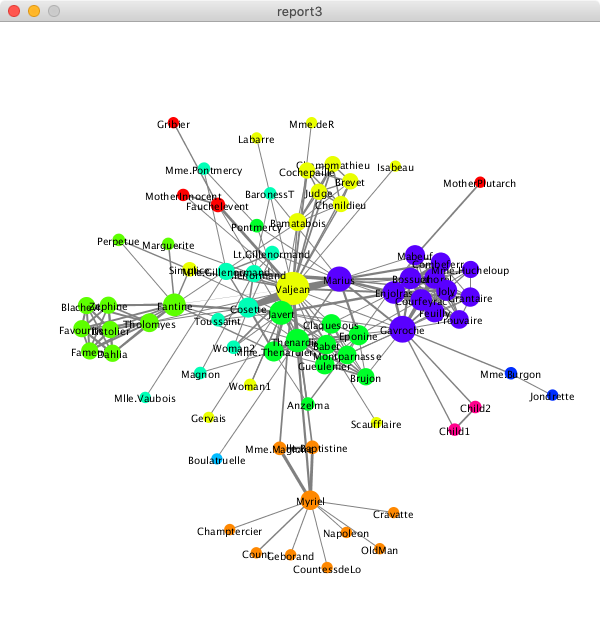
\includegraphics[scale=0.6]{images/resultEx.png}
  \caption{グラフ描画の例}
\end{figure}
\section{結果と考察}
\section{巻末付録}
本稿で使用したソースコード等は以下のリンクから取得できる。必要なら参照いただきたい。
\begin{itemize}
  \item GoogleDrive:\url{https://drive.google.com/drive/folders/1VwNU_T6XjySMzyiFxUrvNyUqlnMTers4?usp=sharing}
  \item GitHubリポジトリ:\url{https://github.com/tsyu12345/data-science2-report3}
\end{itemize}
\end{document}
